\documentclass[aspectratio=169]{beamer}

\usepackage[english]{babel}
\usepackage[utf8x]{inputenc}			
\usepackage{listings}
\usepackage{xcolor}
\usepackage{tikz}
\usetikzlibrary{trees}  % 用於樹狀圖
\lstset{
    language=R,
    basicstyle=\ttfamily\small,
    backgroundcolor=\color{gray!10},
    frame=single,
    breaklines=true,
    showstringspaces=false,
    keywordstyle=\color{blue},
    commentstyle=\color{green!50!black},
    stringstyle=\color{red},
    numbers=none,
    xleftmargin=10pt,
    xrightmargin=10pt,
    framexleftmargin=5pt,
    framexrightmargin=5pt
}

\mode<presentation>						
{
  \usetheme{default}					
  \usecolortheme{default} 			
  \usefonttheme{default}  				
  \setbeamertemplate{caption}[numbered]	
}

\usepackage{graphicx}
\graphicspath{{figure/}}				% Shared figure folder for all labs
\usepackage{booktabs}
\usepackage{hyperref}					
\usepackage{subcaption}  
\usepackage{multicol}
\usepackage{hyperref}

\title{Hypothesis Testing I}	
\author{Rex Shao-Yu Wang}								
\institute{Department of Agronomy, National Taiwan University}				
\date{April 27, 2026}								

\begin{document}

% Title page
\begin{frame}
  \titlepage
\end{frame}

% Outline
\begin{frame}{Outline}
  \tableofcontents
\end{frame}





\section{Hypothesis Testing}
\begin{frame}{Type I and type II errors}
\begin{figure}
    \centering
    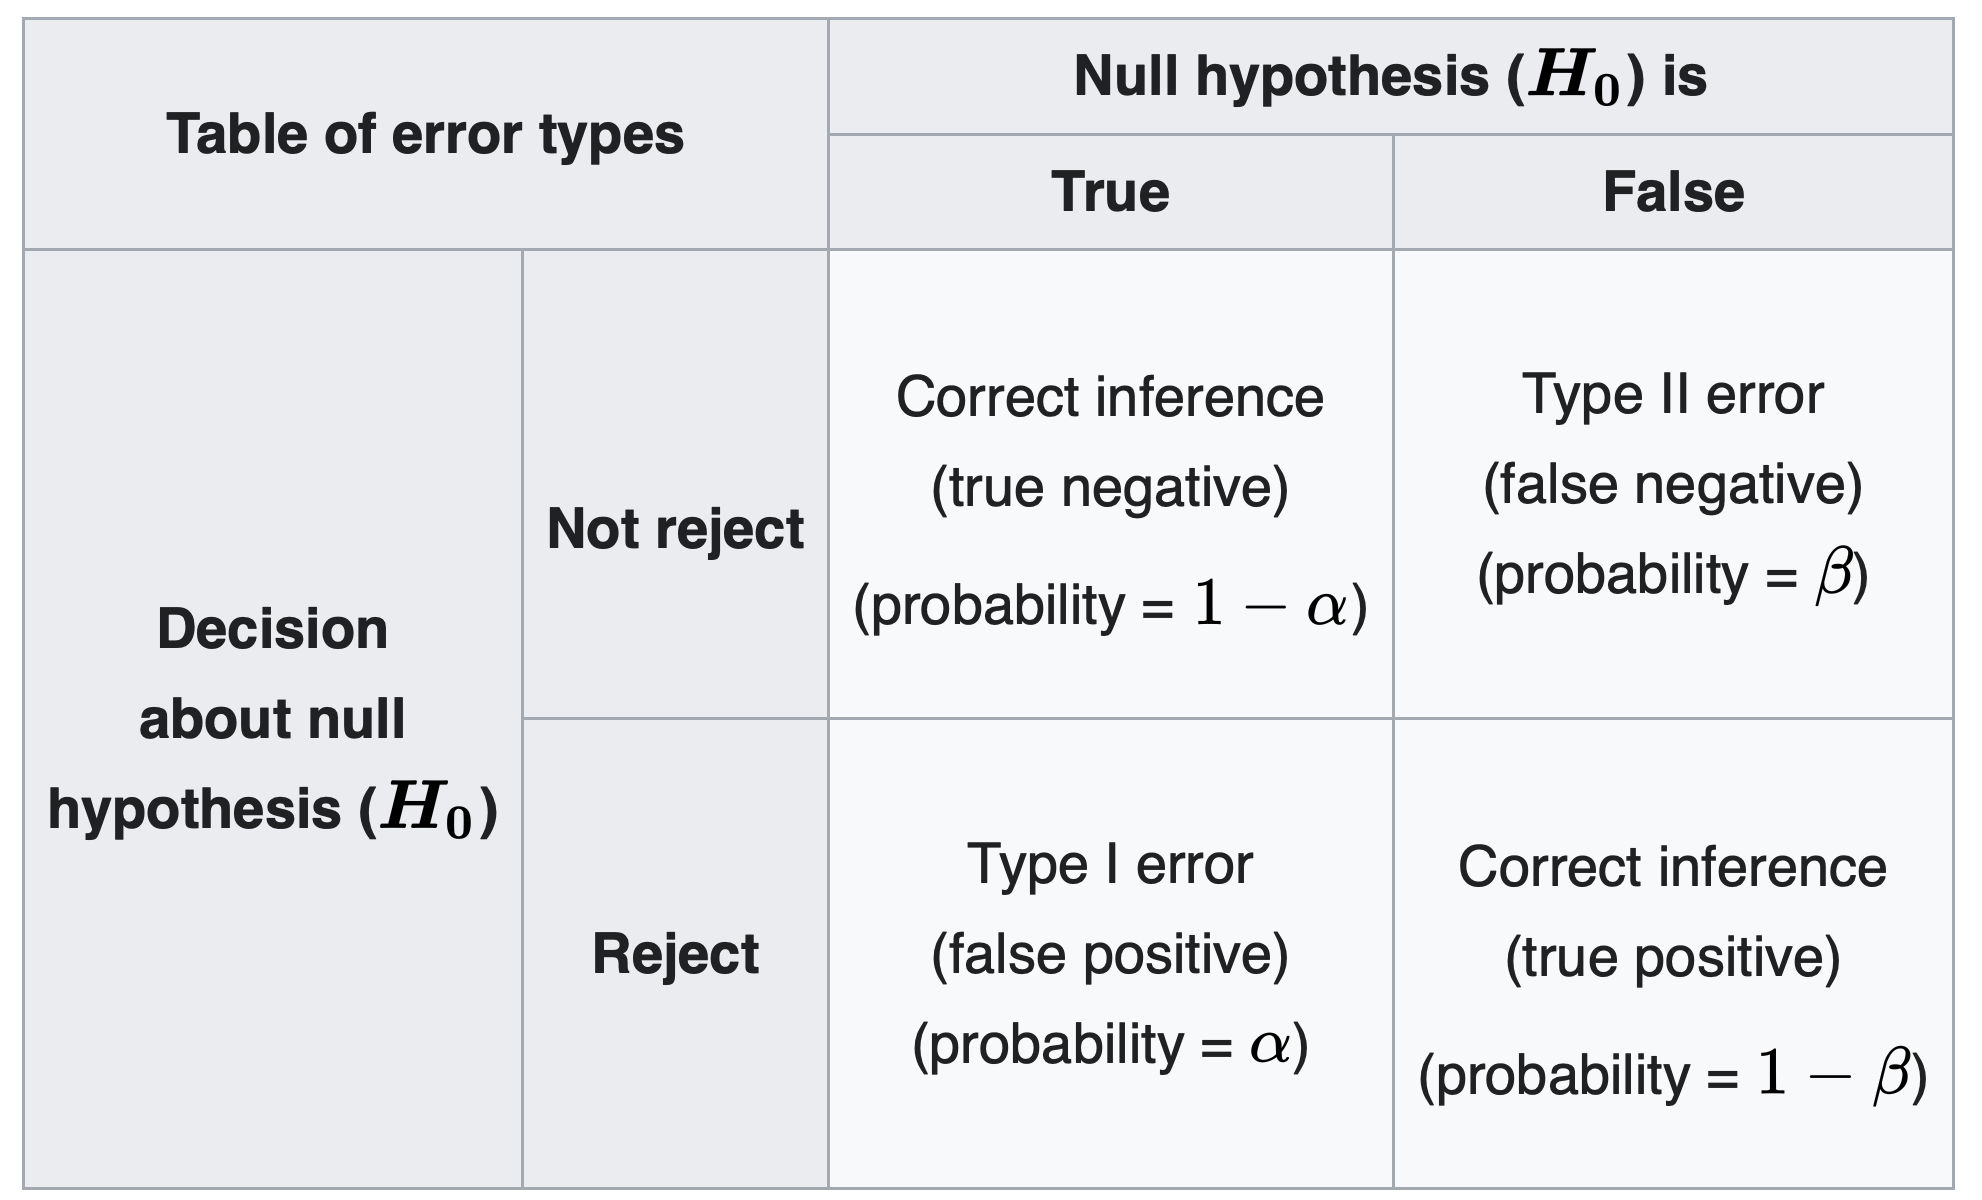
\includegraphics[width=0.85\linewidth]{Screenshot 2026-04-24 at 10.10.26 PM.png}
\end{figure}
\end{frame}


\begin{frame}[fragile]{Procedure for Hypothesis Testing}
\begin{enumerate}
    \item State your null and alternate hypothesis
    \item Define significant level $\alpha$
    \item Decide the test statistic ($Z, T,F $)
    \item Find the rejection region (RR)
    \item Calculate your test statistic and compare with RR
    \item Make a decision whether reject $H_0$ or not
\end{enumerate}
Load the package \texttt{BSDA} before we start.
\begin{lstlisting}
library(BSDA)
\end{lstlisting}
\end{frame}



\begin{frame}[label=dTree]{Types of Hypothesis Testing}
    
\footnotesize 
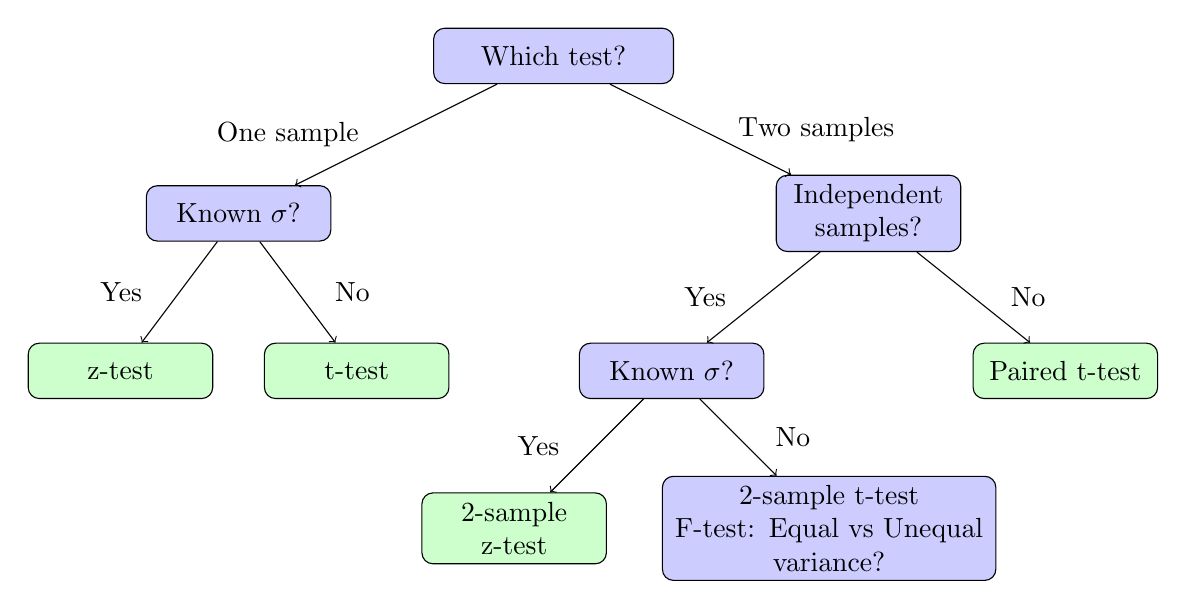
\begin{tikzpicture}[grow=down,level distance=2cm,sibling distance=5cm]
    \tikzstyle{decision} = [rectangle, draw, fill=blue!20, text width=6em, text centered, rounded corners, minimum height=2em]
    \tikzstyle{leaf} = [rectangle, draw, fill=green!20, text width=6em, text centered, rounded corners, minimum height=2em]
    \tikzstyle{edge from parent}=[->, draw]
    \node [decision, text width=8em] (T){Which test?}[sibling distance=8cm] 
    child { node [decision] (S1) {Known $\sigma$?} [sibling distance=3cm] 
        child { node [leaf] {z-test} 
            edge from parent 
            node [left=1em] {Yes} 
        }
        child { node [leaf] {t-test} 
            edge from parent 
            node [right=1em] {No} 
        }
    }
    child { node [decision] (Ind) {Independent samples?} [sibling distance=5cm] 
           child { node [decision] (S2) {Known $\sigma$?}[sibling distance=4cm] 
                child { node [leaf] {2-sample z-test}
                    edge from parent 
                    node [left=1em] {Yes} 
                }
                child { node [decision, text width=4cm] {2-sample t-test\\F-test: Equal vs Unequal\\variance?} [level distance=1.5cm]
                    edge from parent 
                    node [right=1em] {No} 
%                    child { node [leaf, level distance=1cm, text width=4cm] {2-sample t-test} }
                }                
%                child { node  {F-test}                     
%                    edge from parent node [right=1em] {No} }
            }
%        child { %node [decision] {No. Paired samples}
            child { node [leaf] {Paired t-test} 
                edge from parent 
                node [right=1em] {No} 
            }
%        }
    };
    \path (T) to node [left=1em] {One sample} (S1);
    \path (T) to node [right=1em] {Two samples} (Ind);
    \path (Ind) to node [left=1em] {Yes} (S2);
%    \draw (T) -- +(0,-1) |-  {aoeu} (S1);
%    \path (T) |- +(1,-1) -- {oeuid} (S2);
\end{tikzpicture}
\large \centering One-tailed vs Two-tailed
\end{frame}



\section{One sample z-test}
\begin{frame}{One sample z-test}
\begin{itemize}
    \item Hypothesis: 
    \begin{itemize}
        \item Two-sided: $H_0: \mu = \mu_0$ vs. $H_a: \mu \neq \mu_0$ 
        \item One-sided upper-tail: $H_0: \mu \leq \mu_0$ vs. $H_a: \mu > \mu_0$
        \item One-sided lower-tail: $H_0: \mu \geq \mu_0$ vs. $H_a: \mu < \mu_0$
    \end{itemize}
    \item Test Statistic:
    \[
    Z = \frac{\overline{X}-\mu_0}{\frac{\sigma}{\sqrt{n}}} \overset{H_0}{\sim} N(0,1)
    \]
    \item Rejection Region (RR):
    \[
    RR = \{\lvert Z \rvert \ge z_{\frac{\alpha}{2}}\} = \{Z \ge z_{\frac{\alpha}{2}}\ or\ Z \le -z_{\frac{\alpha}{2}}\}
    \]
\end{itemize}
\end{frame}

\begin{frame}[fragile]{One sample z-test}
Let significance level $\alpha = 0.05$, sample mean = 24, known population variance = 100
\begin{itemize}
    \item Two-sided: $H_0 = \mu_0$ vs. $H_a\neq \mu_0$ 
\begin{lstlisting}
z_test <- z.test(data, mu = 24, sigma.x=10, conf.level = 0.95, alternative = "two.sided")
\end{lstlisting}
    \item One-sided upper-tail: $H_0 \leq \mu_0$ vs. $H_a > \mu_0$
\begin{lstlisting}
z_test <- z.test(data, mu = 24, sigma.x=10, conf.level = 0.95, alternative = "greater")
\end{lstlisting}
    \item One-sided lower-tail: $H_0 \ge \mu_0$ vs. $H_a < \mu_0$
\begin{lstlisting}
z_test <- z.test(data, mu = 24, sigma.x=10, conf.level = 0.95, alternative = "less")
\end{lstlisting}
\end{itemize}
\end{frame}



\section{One sample t-test}
\begin{frame}{One sample t-test}
\begin{itemize}
    \item Hypothesis: 
    \begin{itemize}
        \item Two-sided: $H_0: \mu = \mu_0$ vs. $H_a: \mu \neq \mu_0$ 
        \item One-sided upper-tail: $H_0: \mu \leq \mu_0$ vs. $H_a: \mu > \mu_0$
        \item One-sided lower-tail: $H_0: \mu \geq \mu_0$ vs. $H_a: \mu < \mu_0$
    \end{itemize}
    \item Test Statistic:
    \[
    T = \frac{\overline{X}-\mu_0}{\frac{S}{\sqrt{n}}} \overset{H_0}{\sim} t(n-1)
    \]
    \item Rejection Region (RR):
    \[
    RR = \{\lvert T \rvert \ge t_{\frac{\alpha}{2}}\}(n-1) = \{T \ge t_{\frac{\alpha}{2}}(n-1)\ or\ T \le -t_{\frac{\alpha}{2}}(n-1)\}
    \]
\end{itemize}
\end{frame}

\begin{frame}[fragile]{One sample t-test}
Let significance level $\alpha = 0.05$, sample mean = 24, unknown population variance
\begin{itemize}
    \item Two-sided: $H_0 = \mu_0$ vs. $H_a\neq \mu_0$ 
\begin{lstlisting}
t_test <- t.test(data, mu = 24, conf.level = 0.95, alternative = "two.sided")
\end{lstlisting}
    \item One-sided upper-tail: $H_0 \leq \mu_0$ vs. $H_a > \mu_0$
\begin{lstlisting}
t_test <- t.test(data, mu = 24, conf.level = 0.95, alternative = "greater")
\end{lstlisting}
    \item One-sided lower-tail: $H_0 \ge \mu_0$ vs. $H_a < \mu_0$
\begin{lstlisting}
t_test <- t.test(data, mu = 24, conf.level = 0.95, alternative = "less")
\end{lstlisting}
\end{itemize}
\end{frame}



\section{Two sample z-test}
\begin{frame}{Two sample z-test}
\begin{itemize}
    \item Hypothesis:
    \[
    \begin{cases}
    H_0: \mu_1 = \mu_2 \\
    H_A: \mu_1 \neq \mu_2
    \end{cases}
    \]
    \item Test Statistic:
    \[
    Z = \frac{\overline{x_1}-\overline{x_2}-0}{\sqrt{\frac{\sigma_{1}^2}{n_1}+\frac{\sigma_{2}^2}{n_2}}} \overset{H_0}{\sim} N(0,1)
    \]
    \item Rejection Region:
    \[
    RR = \{\lvert Z \rvert \ge z_{\frac{\alpha}{2}}\} = \{Z \ge z_{\frac{\alpha}{2}}\ or\ Z \le -z_{\frac{\alpha}{2}}\}
    \]
\end{itemize}
\end{frame}

\begin{frame}[fragile]{Two sample z-test}
We get two data, data1 and data2, knowing that $\sigma_1 =10 , \sigma_2 = 15$. \\
We want to test whether $\mu_1 = \mu_2$ with significance level $\alpha =0.05$?
\begin{lstlisting}
data1 <- c(27, 24, 18, 29, 30,27)
data2 <- c(23, 28, 20, 19, 35,23)

z_test <- z.test(data1, data2, mu = 0, sigma.x = 10, sigma.y = 15, conf.level = 0.95)
\end{lstlisting}
\end{frame}




\section{Lab Report}
\begin{frame}{Lab Report}
\begin{itemize}
    \item The report file will be in the NTU COOL Assignment section
    \item Submit your file in pdf format
    \item Deadline: 5/3 (Sun) 23:59
    \item Late submission is not accepted
\end{itemize}
\end{frame}

\end{document}




